\documentclass{article}
\usepackage{graphicx} % Required for inserting images
\usepackage{amsmath, amssymb, mathtools, dirtytalk}
\graphicspath{{Images/}}

\setlength{\oddsidemargin}{0in}
\setlength{\textwidth}{6.5in}
\setlength{\topmargin}{-.55in}
\setlength{\textheight}{9in}
\pagestyle{empty}


\title{Optimization HW 4}
\author{Michael Nameika}
\date{February 2023}

\begin{document}

\maketitle

\section*{Section 2.2 Problems}
\textbf{2.} Solve the following linear programs using the simplex method. If the problem is two dimensional, graph the feasible region, and outline the progess of the algorithm.
\begin{itemize}
    \item[(i)] 
    \begin{align*}
        \text{minimize} \:\:\:\: z &= -5x_1 - 7x_2 - 12x_3 + x_4 \\
        \text{subject to} \:\:\:\: &2x_1 + 3x_2 + 2x_3 + x_4 \leq 38\\
        &3x_1 + 2x_2 + 4x_3 - x_4 \leq 55\\
        &x_1,x_2,x_3,x_4 \geq 0.
    \end{align*}
    Adding the slack variables $x_5,x_6 \geq 0$ to the first and second constraints, respectively, we have the problem in standard form with
    \[A = \begin{pmatrix*}[r]
        2 & 3 & 2 & 1 & 1 & 0\\
        3 & 2 & 4 & -1 & 0 & 1
    \end{pmatrix*} \:\:\:\:\: b = \begin{pmatrix}
        38\\
        55
    \end{pmatrix} c = \begin{pmatrix*}[r]
        -5\\
        -7\\
        -12\\
        1\\
        0\\
        0
    \end{pmatrix*}\:\:\:\:\: x = \begin{pmatrix}
        x_1\\
        x_2\\
        x_3\\
        x_4\\
        x_5\\
        x_6
    \end{pmatrix}
    \]
    Choosing the initial basis corresponding to $(x_5,x_6)$ and running a script that implements the simplex method, we find the following:
    \begin{center}
        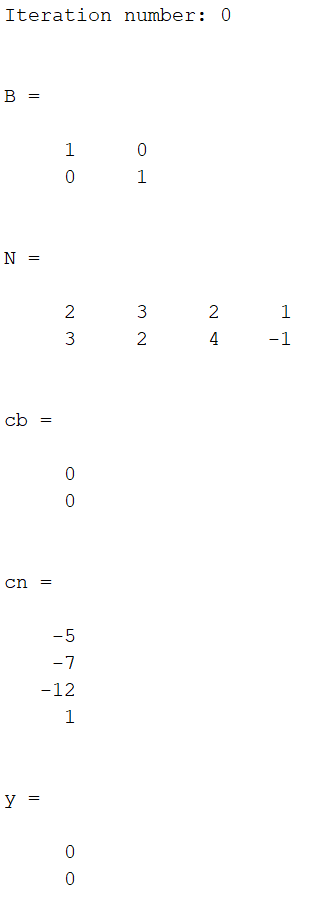
\includegraphics[scale = 0.7]{2_2_i_iter0}
        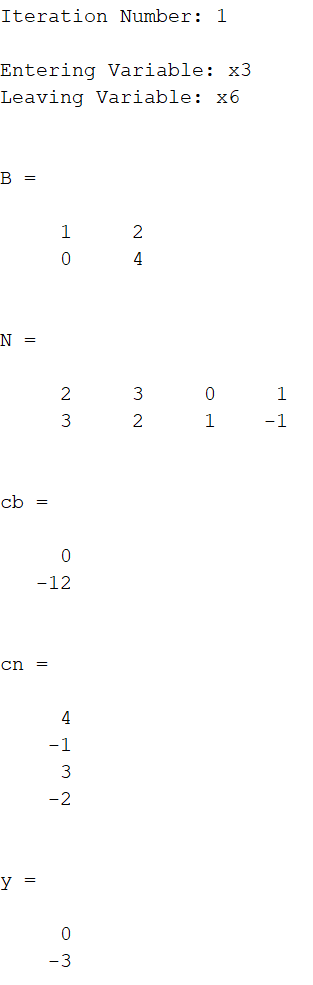
\includegraphics[scale = 0.7]{2_2_i_iter1}
        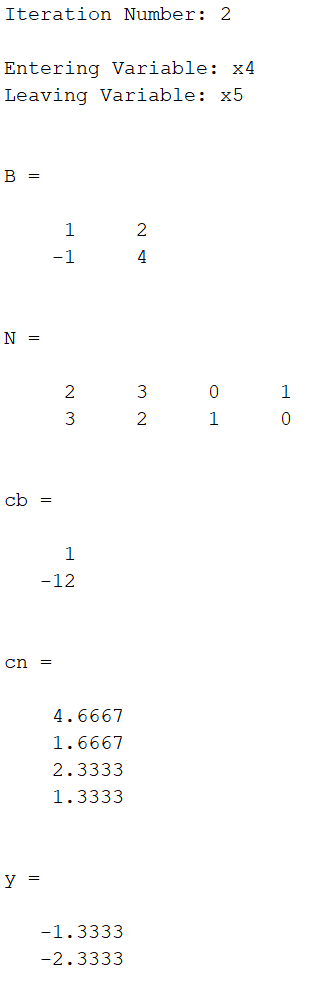
\includegraphics[scale = 0.7]{2_2_i_iter2}
        \newline
        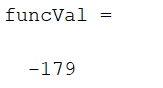
\includegraphics[scale = 1]{2_2_i_min}
    \end{center}
    From the above, we see that the minimal value is $z = -179$.
    \item[(ii)]
    \begin{align*}
        \text{maximize} \:\:\:\: &z = 5x_1 + 3x_2 + 2x_3\\
        \text{subject to} \:\:\: &4x_1 + 5x_2 + 2x_3 + x_4\leq 20\\
        &3x_1 + 4x_2 - x_3 + x_4 \leq 30\\
        &x_1,x_2,x_3,x_4 \geq 0.
    \end{align*}
    Converting the problem to a minimization problem and adding the slack variables $x_5,x_6 \geq 0$ to the first and second constraints, respectively, we have the problem in standard form with
    \[A = \begin{pmatrix*}[r]
        4 & 5 & 2 & 1 & 1 & 0\\
        3 & 4 & -1 & 1 & 0 & 1
    \end{pmatrix*}
    \:\:\:\:\:
    b = \begin{pmatrix}
        20\\
        30
    \end{pmatrix}
    \:\:\:\:\:
    c = \begin{pmatrix*}[r]
        -5\\
        -3\\
        -2\\
        0\\
        0\\
        0
    \end{pmatrix*}
    \:\:\:\:\:
    x = \begin{pmatrix}
        x_1\\
        x_2\\
        x_3\\
        x_4\\
        x_5\\
        x_6
    \end{pmatrix}
    \]
    Choosing the initial basis corresponding to $(x_5,x_6)$ and running the simplex script, we find
    \begin{center}
        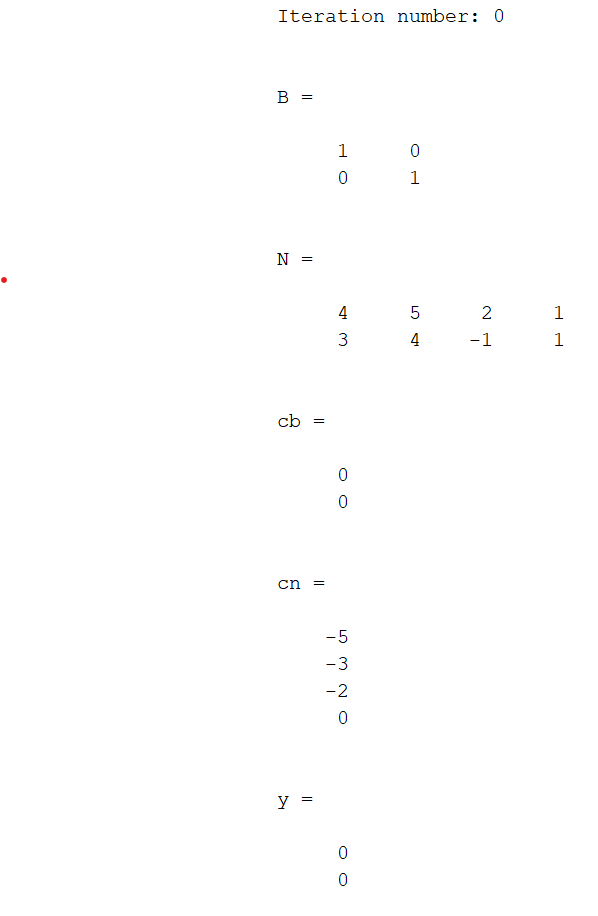
\includegraphics[scale = 0.7]{2_2_ii_iter0}
        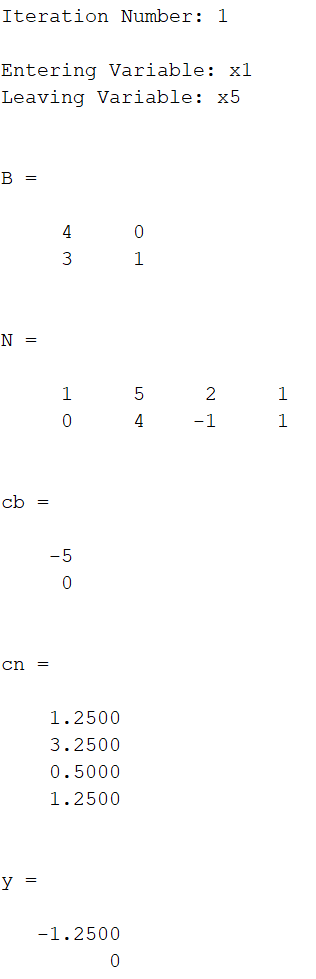
\includegraphics[scale = 0.7]{2_2_ii_iter1}
        \newline
        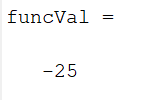
\includegraphics[scale = 1]{2_2_ii_min}
    \end{center}
    From the above, we can see the minimal value is $-z = -25$, and so the maximal value is $z = 25$.

    \item[(v)]
    \begin{align*}
        \text{maximize} \:\:\:\: &z = 7x_1 + 8x_2\\
        \text{subject to} \:\:\: &4x_1 +x_2 \leq 100\\
        &x_1 + x_2 \leq 80\\
        &x_1 \leq 40\\
        &x_1,x_2\geq 0
    \end{align*}
    Since this problem is two dimensional, we may plot the feasible region: 
    \begin{center}
        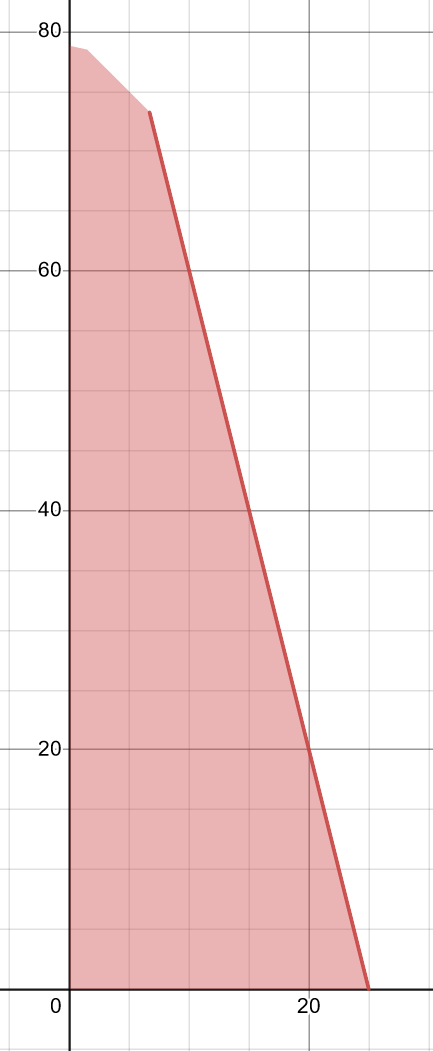
\includegraphics[scale = 0.6]{2_2_v_plot}
    \end{center}
    Converting the problem to a minimization problem and adding the slack variables  $x_3,x_4,x_5 \geq 0$ to the first, second, and third constraints, respectively, we have the problem in standard form with
    \[A = \begin{pmatrix*}
        4 & 1 & 1 & 0 & 0\\
        1 & 1 & 0 & 1 & 0\\
        1 & 0 & 0 & 0 & 1
    \end{pmatrix*}
    \:\:\:\:
    b = \begin{pmatrix}
        100\\
        80\\
        40
    \end{pmatrix}
    \:\:\:\:
    c = \begin{pmatrix*}[r]
        -7\\
        -8\\
        0\\
        0\\
        0
    \end{pmatrix*}
    \]
    Choosing the initial basis corresponding to $(x_4,x_5,x_6)$ and running the simplex script, we find
    \begin{center}
        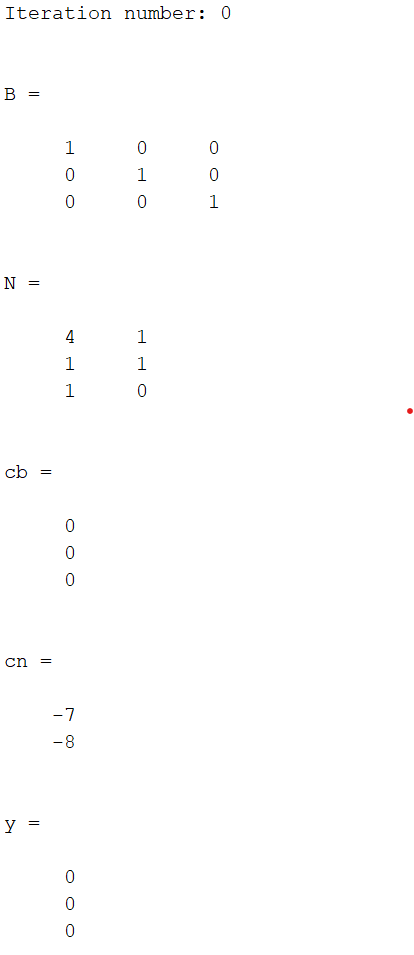
\includegraphics[scale = 0.7]{2_2_v_iter0}
        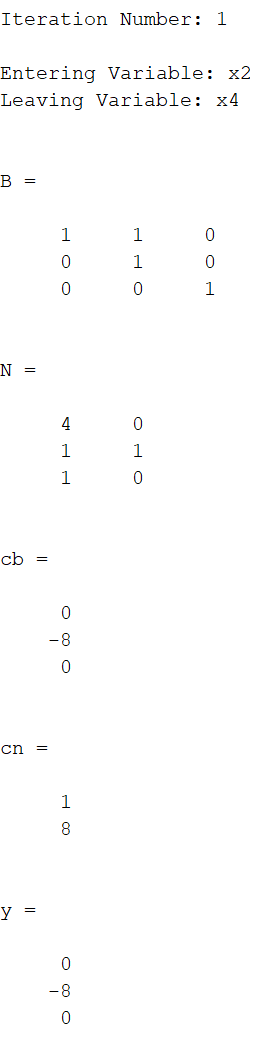
\includegraphics[scale = 0.7]{2_2_v_iter1}
        \newline
        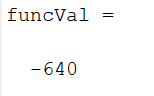
\includegraphics[scale = 1]{2_2_v_min}
    \end{center}
    From the above, we can see the minimal value is $z = -640$, and so the maximal value is $z = 640$.
\end{itemize}

\textbf{3.} Consider the linear program
\begin{align*}
    \text{minimize} \:\:\:\: &z = x_1 - x_2\\
    \text{subject to} \:\:\: &-x_1 + x_2 \leq 1\\
    &x_1 - 2x_2 \leq 2\\
    &x_1,x_2 \geq 0
\end{align*}
Derive an expression for the set of optimal solutions to this problem, and show that this set is unbounded.
\newline\newline
To begin, introduce slack variables $x_3,x_4 \geq 0$ so that the problem is in standard form with 
\[A = \begin{pmatrix*}[r]
    -1 & 1 & 1 & 0\\
    1 & -2 & 0 & 1
\end{pmatrix*}
\:\:\:\:
b = \begin{pmatrix}
    1\\
    2
\end{pmatrix}
\:\:\:\:
c = \begin{pmatrix*}[r]
    1\\
    -1\\
    0\\
    0
\end{pmatrix*}\]
From the system above, performing Gaussian elimination on $(A|b)$ (adding row 1 to row 2 and putting it back into row 2), we find
\[\left(\begin{array}{cccc|c}
    -1 & 1 & 1 & 0 & 1\\
    0 & -1 & 1 & 1 & 3
\end{array}\right)\]
From this, we see that 
\begin{align*}
    x_2 &= x_3 + x_4 - 3\\
    x_1 &= 2x_3 + x_4 - 4
\end{align*}
Then our solution set takes the following form:
\[x = \begin{pmatrix*}[r]
    -4\\
    -3\\
    0\\
    0
\end{pmatrix*} + x_3\begin{pmatrix*}[r]
    2\\
    1\\
    1\\
    0
\end{pmatrix*} + x_4\begin{pmatrix*}[r]
    1\\
    1\\
    0\\
    1
\end{pmatrix*}\]
Notice that $(x_1,x_2)^T = (-4,-3)$ lies on the first constraint, so we may \say{shift} the point to $(0,1)$ so that our solution set takes the form 
\[x = \begin{pmatrix*}[r]
    0\\
    1\\
    0\\
    0
\end{pmatrix*}
\:\:\:\: + 
x_3\begin{pmatrix*}[r]
   2\\
   1\\
   1\\
   0
\end{pmatrix*}
+ \:\:\:\:
x_4\begin{pmatrix*}[r]
    1\\
    1\\
    0\\
    1
\end{pmatrix*}\]
\[x_3,x_4 \geq 0\]. Let $d_1 = (2, 1, 1, 0)^T$ and $d_2 = (1, 1, 0, 1)^T$ and consider $Ad_1$ and $Ad_2$:
\begin{align*}
    Ad_1 &= \begin{pmatrix*}[r]
        -1 & 1 & 1 & 0\\
        1 & -2 & 0 & 1
    \end{pmatrix*}
    \begin{pmatrix*}[r]
        2\\
        1\\
        1\\
        0
    \end{pmatrix*}\\
    &= 
    \begin{pmatrix*}
        0\\
        0
    \end{pmatrix*}
\end{align*}

\begin{align*}
    Ad_2 &= \begin{pmatrix*}[r]
        -1 & 1 & 1 & 0\\
        1 & -2 & 0 & 1
    \end{pmatrix*}
    \begin{pmatrix*}[r]
        1\\
        1\\
        0\\
        1
    \end{pmatrix*}\\
    &= \begin{pmatrix}
        0\\
        0
    \end{pmatrix}
\end{align*}
So we have that both $d_1$ and $d_2$ are directions of unboundedness, meaning that this problem is unbounded.
\newline\newline\newline
\text{11.} Solve the linear programs in Exercise 2.2 using the tableau.
\newline\newline
See attached work.

\end{document}
